% Q22: the source shows the incircle, its first tangent circle, and the next small circle near B.
% A normalized side length of 6 is used only to lay out the schematic.
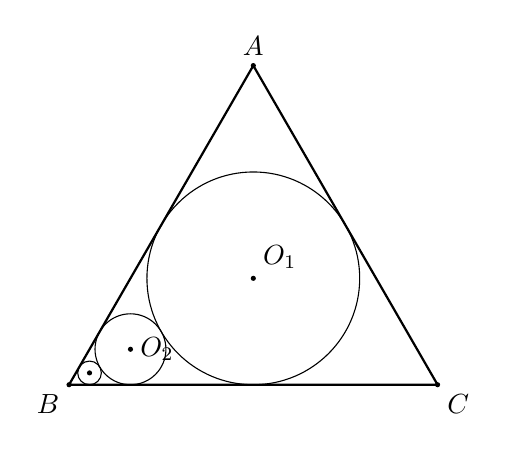
\begin{tikzpicture}[scale=0.78,line cap=round,line join=round]
  \coordinate (A) at (3,5.19615);
  \coordinate (B) at (0,0);
  \coordinate (C) at (6,0);
  \coordinate (Oone) at (3,1.73205);
  \coordinate (Otwo) at (1,0.57735);
  \coordinate (Othree) at (0.33333,0.19245);
  \draw[thick] (A)--(B)--(C)--cycle;
  \draw (Oone) circle (1.73205);
  \draw (Otwo) circle (0.57735);
  \draw (Othree) circle (0.19245);
  \fill (A) circle (1.2pt) node[above] {$A$};
  \fill (B) circle (1.2pt) node[below left] {$B$};
  \fill (C) circle (1.2pt) node[below right] {$C$};
  \fill (Oone) circle (1.2pt) node[above right] {$O_1$};
  \fill (Otwo) circle (1.2pt) node[right] {$O_2$};
  \fill (Othree) circle (1.2pt);
\end{tikzpicture}
